%%%%%%%%%%%%%%%%%%%%%%%%%%%%%%%%%%%%%%%%%%%%%%%%%%%%%%%%%%%%%%%%%%%%%%%%%%%%%%%%%%%%%%%%%%%%%%%%%%%%%%%%%%%%%%%%%%%%
%%% Template for Reproduced Sound 2020 
%%% Release 21/09/2020
%%%	Developed by Prof. William D'Andrea Fonseca (Acoustical Engineering, UFSM, Brazil)
%%% will.fonseca@eac.ufsm.br
%%%%%%%%%%%%%%%%%%%%%%%%%%%%%%%%%%%%%%%%%%%%%%%%%%%%%%%%%%%%%%%%%%%%%%%%%%%%%%%%%%%%%%%%%%%%%%%%%%%%%%%%%%%%%%%%%%%%
\documentclass[10pt, a4paper, oneside]{article}
%%%%%%%%%%%%%%%%%%%%%%%%%%%%%%%%%%%%%%%%%%%%%%%%%%%%
%%% Input
\usepackage[utf8]{inputenc} 
%%%%%%%%%%%%%%%%%%%%%%%%%%%%%%%%%%%%%%%%%%%%%%%%%%%%
\usepackage{ReproducedSound}  %%% Basic configurations
%%%%%%%%%%%%%%%%%%%%%%%%%%%%%%%%%%%%%%%%%%%%%%%%%%%%%%%%%%%%%%%%%%%%%%%%%%%%%%%%%%%%%%%%%%%%%%%%%%%%%%%%%%%%%%%%%%%%
%%% Paper data

\CompleteTitle{SPEECH RESEARCH AT THE UNIVERSITY OF ATLANTIS {\#\#} $[$3 LINES FOR TITLE, SOME MAY BE EMPTY, STYLE, LEFT JUSTIFIED 16 POINT ARIAL BOLD UPPERCASE$]$}

\Authors{B.~Long; G.~G.~Small; R.~U.~Little; M.~W.~Short} 

\newcommand{\AuthorsTable}{
\noindent \hspace{-3mm}
\begin{tabular}{L{2.6cm} l}
%%%%%%%%%%%%%%%%%%%%%%%%%%%%%%%%% Authors and Affiliations %%%%%%%%%%%%%%%%%%%%%%%%%%%%%%%%%%%%%%%%%%%%%%%%%%%%%%%%%%%%%%%%%%%%%
							B.~Long & Underwater Listening Devices, Newtown, Michigan, USA\\[1.2pt] 
							G.~G.~Small &  Underwater Listening Devices, Newtown, Michigan, USA\\[1.2pt] 
              R.~U.~Little & South West Coast Associates, Atlantis City, Lost Islands\\[1.2pt] 
							M.~W.~Short & Underwater Listening Devices, Newtown, Michigan, USA\\[1.2pt] 
%%%%%%%%%%%%%%%%%%%%%%%%%%%%%%%%%%%%%%%%%%%%%%%%%%%%%%%%%%%%%%%%%%%%%%%%%%%%%%%%%%%%%%%%%%%%%%%%%%%%%%%%%%%%%%%%%%%%%%%%%%%%%%%%							
\end{tabular}\\
\textit{(Authors style, 10 point Arial, Use 6 lines, of which some may be empty)}
}							

\EmailAuthor{b.long@reproducedsound.ac.uk}

\Abstract{An increasing awareness of the environmental noise problems means that a better knowledge of the effects of weather on sound propagation is necessary. Measured sound pressure levels owe as much to near-surface weather as to ground shape and impedance and factors such as source and receiver heights and locations. Wind and temperature gradients in the atmosphere cause refraction that can increase or decrease sound pressure levels significantly. However, the variability in meteorological parameters over the propagation path and measurement duration creates uncertainties in the measurement of temperature, wind speed and direction in practical situations. To investigate these uncertainties experiments were performed using an omni-directional point source over flat grassland and tarmac and a barrier. These measurements were specifically performed at distances typical to community noise problems. However, automatic weather stations, SODAR and LIDAR were used to simultaneously collect detailed meteorological information at a number of locations along the propagation path. These detailed range-dependent meteorological and acoustical measurements are reported here, together with correlations between the meteorological and propagation data. Having assessed the difficulties arising from the effects of meteorology, suggestions are made concerning the practical measurement and prediction of noise levels.} 

%% Optional for metadata %%%%%%%%%%%%%%%%%%%%%%%%%%%%%%%%%%%%%%%%%%%%%%%%%%%%%%%
\Keywords{word, word} \PACS{Code} % PACS codes in https://asa.scitation.org/pb-assets/files/publications/jas/Acoustics_PACS-1548697226033.pdf
\MakePDFmetadata
%%%%%%%%%%%%%%%%%%%%%%%%%%%%%%%%%%%%%%%%%%%%%%%%%%%%%%%%%%%%%%%%%%%%%%%%%%%%%%%%%%%%%%%%%%%%%%%%%%%%%%%%%%%%%%%%%%%%
%%%%%%%%%%%%%%%%%%%%%%%%%%%%%%%%%%%%%%%%%%%%%%%%%%%%%%%%%%%%%%%%%%%%%%%%%%%%%%%%%%%%%%%%%%%%%%%%%%%%%%%%%%%%%%%%%%%%
\begin{document} \setcounter{page}{1} \pagestyle{plain}
%%%%%%%%%%%%%%%%%%%%%%%%%%%%%%%%%%%%%%%%%%%%%%%%%%%%%%%%%%%%%%%%%%%%%%%%%%%%%%%%%%%%%%%%%%%%%%%%%%%%%%%%%%%%%%%%%%%%
%%%%%%%%%%%%%%%%%%%%%%%%%%%%%%%%%%%%%%%%%%%%%%%%%%%%%%%%%%%%%%%%%%%%%%%%%%%%%%%%%%%%%%%%%%%%%%%%%%%%%%%%%%%%%%%%%%%%
%% Title
{\fontsize{16}{18.5}\selectfont\bfseries \MakeUppercase \CompleteTitlePaper \par}
%%%%%%%%%%%%%%%%%%%%%%%%%%%%%%%%%%%%%%%%%%%%%%%%%%%%%%%%%%%%%%%%%%%%%%%%%%%%%%%%%%%%%%%%%%%%%%%%%%%%%%%%%%%%%%%%%%%%
%% Authors
\AuthorsTable \vspace{0.2\baselineskip} % Adjust depending on the number of authors
%%%%%%%%%%%%%%%%%%%%%%%%%%%%%%%%%%%%%%%%%%%%%%%%%%%%%%%%%%%%%%%%%%%%%%%%%%%%%%%%%%%%%%%%%%%%%%%%%%%%%%%%%%%%%%%%%%%%
%%%%%%%%%%%%%%%%%%%%%%%%%%%%%%%%%%%%%%%%%%%%%%%%%%%%%%%%%%%%%%%%%%%%%%%%%%%%%%%%%%%%%%%%%%%%%%%%%%%%%%%%%%%%%%%%%%%%
%%% Text
\fontsize{10}{11}\selectfont 
%\vspace{1\baselineskip}
%%%%%%%%%%%%%%%%%%%%%%%%%%%%%%%%%%%%%%%%%%%%%%%%%%%%%%%%%%%%%%%%%%%%%%%%%%%%%%%%%%%%%%%%%%%%%%%%%%%%%%%%%%%%%%%%%%%%
%%%%%%%%%%%%%%%%%%%%%%%%%%%%%%%%%%%%%%%%%%%%%%%%%%%%%%%%%%%%%%%%%%%%%%%%%%%%%%%%%%%%%%%%%%%%%%%%%%%%%%%%%%%%%%%%%%%%
%%% PAPER
%%%%%%%%%%%%%%%%%%%%%%%%%%%%%%%%%%%%%%%%%%%%%%%%%%%%%%%%%%%%%%%%%%%%%%%%%%%%%%%%%%%%%%%%%%%%%%%%%%%%%%%%%%%%%%%%%%%%
%%%%%%%%%%%%%%%%%%%%%%%%%%%%%%%%%%%%%%%%%%%%%%%%%%%%%%%%%%%%%%%%%%%%%%%%%%%%%%%%%%%%%%%%%%%%%%%%%%%%%%%%%%%%%%%%%%%%
\section{Introduction}

\#\#[\textit{heading 1, 14~pt Arial, upper case, 10~cm from top margin, 10~pt blank line below}]

\#\#[Please ensure that the paper size is set to A4 and not letter size, especially US delegates. Normal text is 10~pt Arial, fully justified left and right, normal text style, leave 2$\times$10 point lines spaces before next heading. The page margins are left 27~mm, right 27~mm, bottom 25~mm and top 40~mm]. 

This paper describes recent speech research activities at the University of Atlantis. The practical application of these requirements can however cause a number of problems due to the very nature of the agent that has to be investigated. This follows from the two basic facts that most voices generate levels that vary with time and that sound waves attenuate as the distance from the source increases. Consequently, the noise climate in which any individual vocalises is determined by both the noise output of any appliances in their vicinity and how they move relative to them. It is a prerequisite for an accurate assessment of any given situation therefore, to take account of the variation of noise levels in the locality.



%%%%%%%%%%%%%%%%%%%%%%%%%%%%%%%%%%%%%%%%%%%%%%%%%%%%%%%%%%%%%%%%%%%%%%%%%%%%%%%%%%%%%%%%%%%%%%%%%%%%%%%%%%%%%%%%%%%%
%%%%%%%%%%%%%%%%%%%%%%%%%%%%%%%%%%%%%%%%%%%%%%%%%%%%%%%%%%%%%%%%%%%%%%%%%%%%%%%%%%%%%%%%%%%%%%%%%%%%%%%%%%%%%%%%%%%%
\section{Research Prior to 1974}

\#\#[\textit{Outlined numbered, text starts 1.25~cm from left margin}]

%%%%%%%%%%%%%%%%%%%%%%%%%%%%%%%%%%%%%%%%%%%%%%%%%%%%%%%%%%%%%%%%%%%%%%%%%%%%%%%%%%%%%%%%%%%%%%%%%%%%%%%%
\subsection{Speech Analysis Research}

\#\#[\textit{Heading2 Capitalised 12~pt bold Arial, 10~pt blank line below}]

The regulations identity noise exposure (also known as noise dose) as the parameter of the risk and this in turn is a function of both the noise level in dB(A) and exposure time. $^*h'$ is the product of these two variables that has to be contained if the risk is to be controlled, hence as noise level increases the exposure duration must be reduced to balance the risk. Strictly speaking the deafness risk is proportional to the noise energy emission into the ear, with a doubling of the energy level being an increment of 3 dB(A) on the logarithmic decibel scale. For every 3 dB(A) change in the noise level therefore, there must be a corresponding halving or doubling of the exposure duration. \#\#[One 10pt blank lines between paragraphs].

These variations with time are dealt with by the use of the ``equivalent continuous'' noise level. As it's name suggests this is a method of calculating a single steady level that has both the same noise energy level and duration as the varying time pattern under consideration. It is given the symbol LAq,t, Level of the A weighted equivalent continuous sound averaged over a specified time, and refers to the level at any one particular location. The LAeq,t value can therefore be read as a steady level and compared against the permitted exposure times given in Figure~\ref{fig:beamforming}.

\clearpage
The regulations identity noise exposure (also known as noise dose) as the parameter of the risk and this in turn is a function of both the noise level in dB(A) and exposure time. $^*h'$ is the product of these two variables that has to be contained if the risk is to be controlled, hence as noise level increases the exposure duration must be reduced to balance the risk. Strictly speaking the deafness risk is proportional to the noise energy emission into the ear, with a doubling of the energy level being an increment of 3 dB(A) on the logarithmic decibel scale. For every 3 dB(A) change in the noise level therefore, there must be a corresponding halving or doubling of the exposure duration. \#\#[One 10pt blank lines between paragraphs].


\begin{figure}[H]
	\centering
	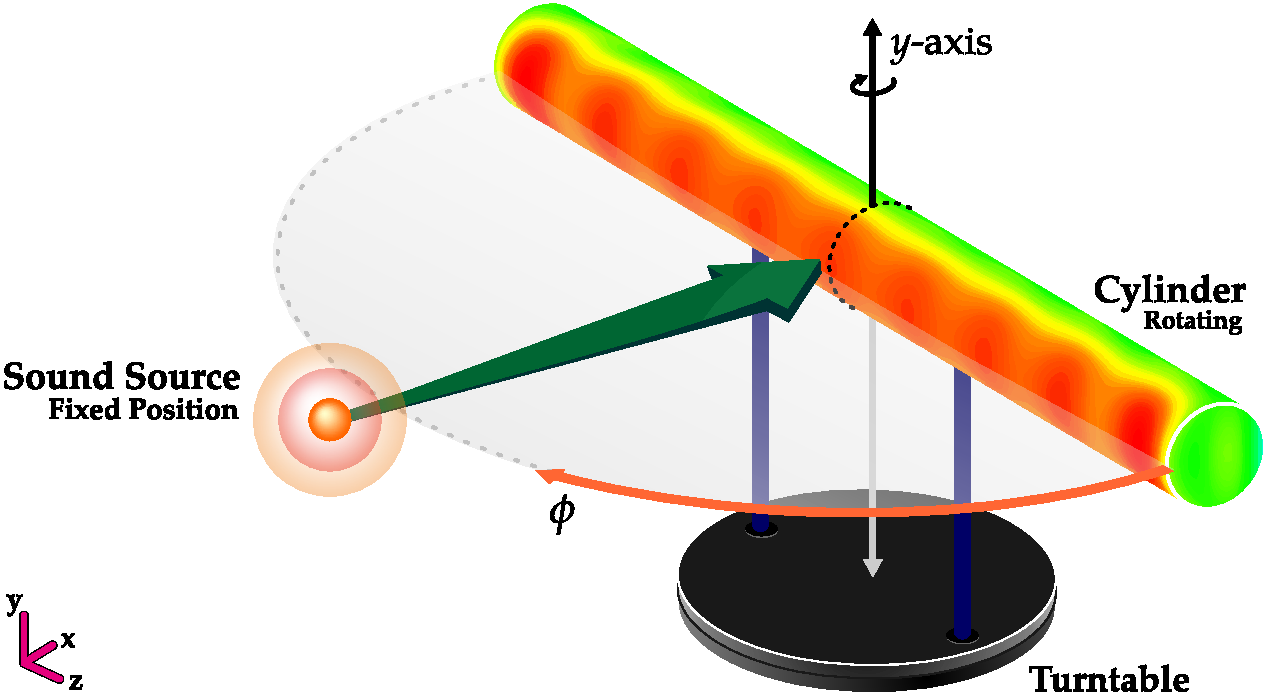
\includegraphics[width=0.75\linewidth]{figs/Measurement-Scheme-Fonseca-2013.pdf}%
	\caption{Just an example of figure (extracted from Fonseca\cite{Fonseca-2013}).}%
	\label{fig:beamforming}%
\end{figure}

%%%%%%%%%%%%%%%%%%%%%%%%%%%%%%%%%%%%%%%%%%%%%%%%%%%%%%%%%%%%%%%%%%%%%%%%%%%%%%%%%%%%%%%%%%%%%%%%%%%%%%%%
\subsubsection{Development}

\#\#[\textit{Heading 3, 12~pt bold Arial Capitalise. Leave 1 $\times$ 10~pt blank line below}]

\#\#[Avoid further heading levels]

\#\#[please add the footer (do not add page numbers)]

The equation
\begin{equation}
p(t) = \frac{s\left( t-\frac{R(t)}{c} \right )}{\; 4\pi R(t)(1-M\,\text{cos}[\theta(t)])^2 \;} \cdot \int_a^b H(t) \dt t\,
\label{eq:example}
\end{equation}
%
is just for testing.

%%%%%%%%%%%%%%%%%%%%%%%%%%%%%%%%%%%%%%%%%%%%%%%%%%%%%%%%%%%%%%%%%%%%%%%%%%%%%%%%%%%%%%%%%%%%%%%%%%%%%%%%%%%%%%%%%%%%
%%%%%%%%%%%%%%%%%%%%%%%%%%%%%%%%%%%%%%%%%%%%%%%%%%%%%%%%%%%%%%%%%%%%%%%%%%%%%%%%%%%%%%%%%%%%%%%%%%%%%%%%%%%%%%%%%%%%
\section{Other Style Comments}

\textit{(text starts at 40~mm from top of page)}

\#\# Header should read [``Proceedings of the Institute of Acoustics'']

\#\#[Figures can be reproduced in colour or black and white but bear in mind that if they use colour, the figures may become unintelligible if photocopied in black and white.]

\#\#[Papers will normally be 8 pages long, we will accept up to 12 pages. You should also provide an abstract to the Institute of Acoustics if you have not already done so.]

\#\#[Papers to be emailed to linda.canty@ioa.org.uk.]

\#\#[Figure should be numbered, e.g. Figure~\ref{fig:beamforming}, with captions in 10~pt Arial]

\#\#[References should be numbered in superscript and appear at the end of the paper\cite{Mareze-2019,Steeneken,cox2001extracting,Haykin,arial}.


%%%%%%%%%%%%%%%%%%%%%%%%%%%%%%%%%%%%%%%%%%%%%%%%%%%%%%%%%%%%%%%%%%%%%%%%%%%%%%%%%%%%%%%%%%%%%%%%%%%%%%%%%%%%%%%%%%%%
%%%%%%%%%%%%%%%%%%%%%%%%%%%%%%%%%%%%%%%%%%%%%%%%%%%%%%%%%%%%%%%%%%%%%%%%%%%%%%%%%%%%%%%%%%%%%%%%%%%%%%%%%%%%%%%%%%%%
%%% References
\renewcommand{\refname}{References} \renewcommand{\bibname}{References} 
\bibliographystyle{unsrtnat3}
\bibliography{references}
%%%%%%%%%%%%%%%%%%%%%%%%%%%%%%%%%%%%%%%%%%%%%%%%%%%%%%%%%%%%%%%%%%%%%%%%%%%%%%%%%%%%%%%%%%%%%%%%%%%%%%%%
%%%%%%%%%%%%%%%%%%%%%%%%%%%%%%%%%%%%%%%%%%%%%%%%%%%%%%%%%%%%%%%%%%%%%%%%%%%%%%%%%%%%%%%%%%%%%%%%%%%%%%%%
%% Abstract and bio [not standard] 
%\clearpage
%\rule{\linewidth}{.2pt}%
%%%%%%%%%%%%%%%%%%%%%%%%%%%%%%%%%%%%%%%%%%%%%%%%%%%%%%%%%%%%%%%%%%%%%%%%%%%%%%%%%%%%%%%%%%%%%%%%%%%%%%%%%%%%%%%%%%%%%
%%% Template for Reproduced Sound 2020 
%%% Release 21/09/2020
%%%	Developed by Prof. William D'Andrea Fonseca (Acoustical Engineering, UFSM, Brazil)
%%% will.fonseca@eac.ufsm.br
%%%%%%%%%%%%%%%%%%%%%%%%%%%%%%%%%%%%%%%%%%%%%%%%%%%%%%%%%%%%%%%%%%%%%%%%%%%%%%%%%%%%%%%%%%%%%%%%%%%%%%%%%%%%%%%%%%%%
%%% Abstract page
%%%%%%%%%%%%%%%%%%%%%%%%%%%%%%%%%%%%%%%%%%%%%%%%%%%%%%%%%%%%%%%%%%%%%%%%%%%%%%%%%%%%%%%%%%%%%%%
\thispagestyle{empty}
%% Abstract format -> Font size:	10pt | Text: Justified | Words:	150 | No diagrams or photographs please
%% Title
{\fontsize{10}{12}\selectfont \bfseries \MakeUppercase \CompleteTitlePaper \par}

\fontsize{10}{12}\selectfont
%% Authors
\AuthorsTable

\EmailAuthorPaper

%\vspace{10pt}

%% Abstract

\AbstractPaper

Keywords: \KeywordsPaper\xspace.

PACS: \PACSPaper\par

%% EOF %%%%%%%%%%%%%%%%%%%%%%%%%%%%%%%%%%%%%%%%%%%%%%%%%%%%%%%%%%%%%%%%%%%%%%%%%%%%%%%%%%%%%%%%

%
%\rule{\linewidth}{.2pt}%
%%%%%%%%%%%%%%%%%%%%%%%%%%%%%%%%%%%%%%%%%%%%%%%%%%%%%%%%%%%%%%%%%%%%%%%%%%%%%%%%%%%%%%%%%%%%%%%%%%%%%%%%%%%%%%%%%%%%%
%%% Template for Reproduced Sound 2020 
%%% Release 21/09/2020
%%%	Developed by Prof. William D'Andrea Fonseca (Acoustical Engineering, UFSM, Brazil)
%%% will.fonseca@eac.ufsm.br
%%%%%%%%%%%%%%%%%%%%%%%%%%%%%%%%%%%%%%%%%%%%%%%%%%%%%%%%%%%%%%%%%%%%%%%%%%%%%%%%%%%%%%%%%%%%%%%%%%%%%%%%%%%%%%%%%%%%
%%% Bio page
%%%%%%%%%%%%%%%%%%%%%%%%%%%%%%%%%%%%%%%%%%%%%%%%%%%%%%%%%%%%%%%%%%%%%%%%%%%%%%%%%%%%%%%%%%%%%%%
%% 150 word biography for each author
\thispagestyle{empty}
\fontsize{10}{12}\selectfont
%% Authors

\textit{Biography:}

\textbf{B. LONG} is a Senior Lecturer in Media Technology with Oxford Brookes University, specialising in audio. He has extensive real world practice of audio engineering, both in music production, sound art installations, and in live and recorded multichannel surround sound productions. He is a member of the Audio Engineering Society, the Institute of Sound and Communications Engineers, and the Institute of Acoustics.  

\textbf{G. G. SMALL} is a Senior Lecturer in Media Technology with Oxford Brookes University, specialising in audio. He has extensive real world practice of audio engineering, both in music production, sound art installations, and in live and recorded multichannel surround sound productions. He is a member of the Audio Engineering Society, the Institute of Sound and Communications Engineers, and the Institute of Acoustics.  

\textbf{R. U. LITTLE} is a Senior Lecturer in Media Technology with Oxford Brookes University, specialising in audio. He has extensive real world practice of audio engineering, both in music production, sound art installations, and in live and recorded multichannel surround sound productions. He is a member of the Audio Engineering Society, the Institute of Sound and Communications Engineers, and the Institute of Acoustics.  


\textbf{M. W. SHORT} is a Senior Lecturer in Media Technology with Oxford Brookes University, specialising in audio. He has extensive real world practice of audio engineering, both in music production, sound art installations, and in live and recorded multichannel surround sound productions. He is a member of the Audio Engineering Society, the Institute of Sound and Communications Engineers, and the Institute of Acoustics.  
%% EOF %%%%%%%%%%%%%%%%%%%%%%%%%%%%%%%%%%%%%%%%%%%%%%%%%%%%%%%%%%%%%%%%%%%%%%%%%%%%%%%%%%%%%%%%
  % 150 word biography for each author
%%%%%%%%%%%%%%%%%%%%%%%%%%%%%%%%%%%%%%%%%%%%%%%%%%%%%%%%%%%%%%%%%%%%%%%%%%%%%%%%%%%%%%%%%%%%%%%%%%%%%%%%
%%%%%%%%%%%%%%%%%%%%%%%%%%%%%%%%%%%%%%%%%%%%%%%%%%%%%%%%%%%%%%%%%%%%%%%%%%%%%%%%%%%%%%%%%%%%%%%%%%%%%%%%
\end{document}
% EOF %%%%%%%%%%%%%%%%%%%%%%%%%%%%%%%%%%%%%%%%%%%%%%%%%%%%%%%%%%%%%%%%%%%%%%%%%%%%%%%%%%%%%%%%%%%%%%%%%%